\documentclass[border=5pt]{standalone}

% Required for Bengali text rendering and math
\usepackage{fontspec}
\usepackage{amsmath}
\usepackage{tikz}

\setmainfont{Noto Sans Bengali}

\begin{document}

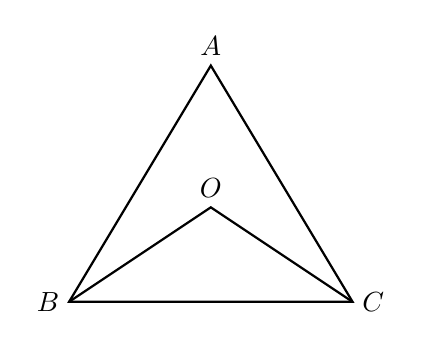
\begin{tikzpicture}[scale=1.2]
    % Coordinates for Triangle ABC and center O
    \coordinate (A) at (1.5, 2.5);
    \coordinate (B) at (0, 0);
    \coordinate (C) at (3, 0);
    \coordinate (O) at (1.5, 1.0);

    % Draw the main triangle
    \draw[thick] (A) -- (B) -- (C) -- cycle;

    % Draw lines connecting to O (Internal Bisectors style)
    \draw[thick] (B) -- (O) -- (C);

    % Label the points using Math Mode
    \node[above] at (A) {$A$};
    \node[left] at (B) {$B$};
    \node[right] at (C) {$C$};
    \node[above] at (O) {$O$};

\end{tikzpicture}

\end{document}
